% Provenance (never printed): cycle 2 "Questionner le monde" (states of water in
% weather phenomena; daily observation), see sources/book1/PROVENANCE.md.
% Book 1, grade 1, chapter 1. No real-world number in this chapter.
\chapter{Mengamati Cuaca}\label{ch:g1:watching-the-weather}

Hari masih pagi sekali. Lena bangun, naik ke kursi di dekat jendela
kamarnya, lalu melihat ke luar. Langit berwarna kelabu. Tetes-tetes air
kecil mengalir di kaca. Atap-atap rumah di seberang jalan basah dan
mengilap, dan pohon di kebun meneteskan air.

``Hari ini aku pakai baju apa, ya?'' tanyanya.

Untuk menjawabnya, Lena tidak memerlukan buku atau mesin. Ia cukup melihat
ke luar jendela. Jendela itu adalah stasiun \omterm{def:g1:watching-the-weather:weather}{cuaca} pertamanya.

\begin{omfigure}
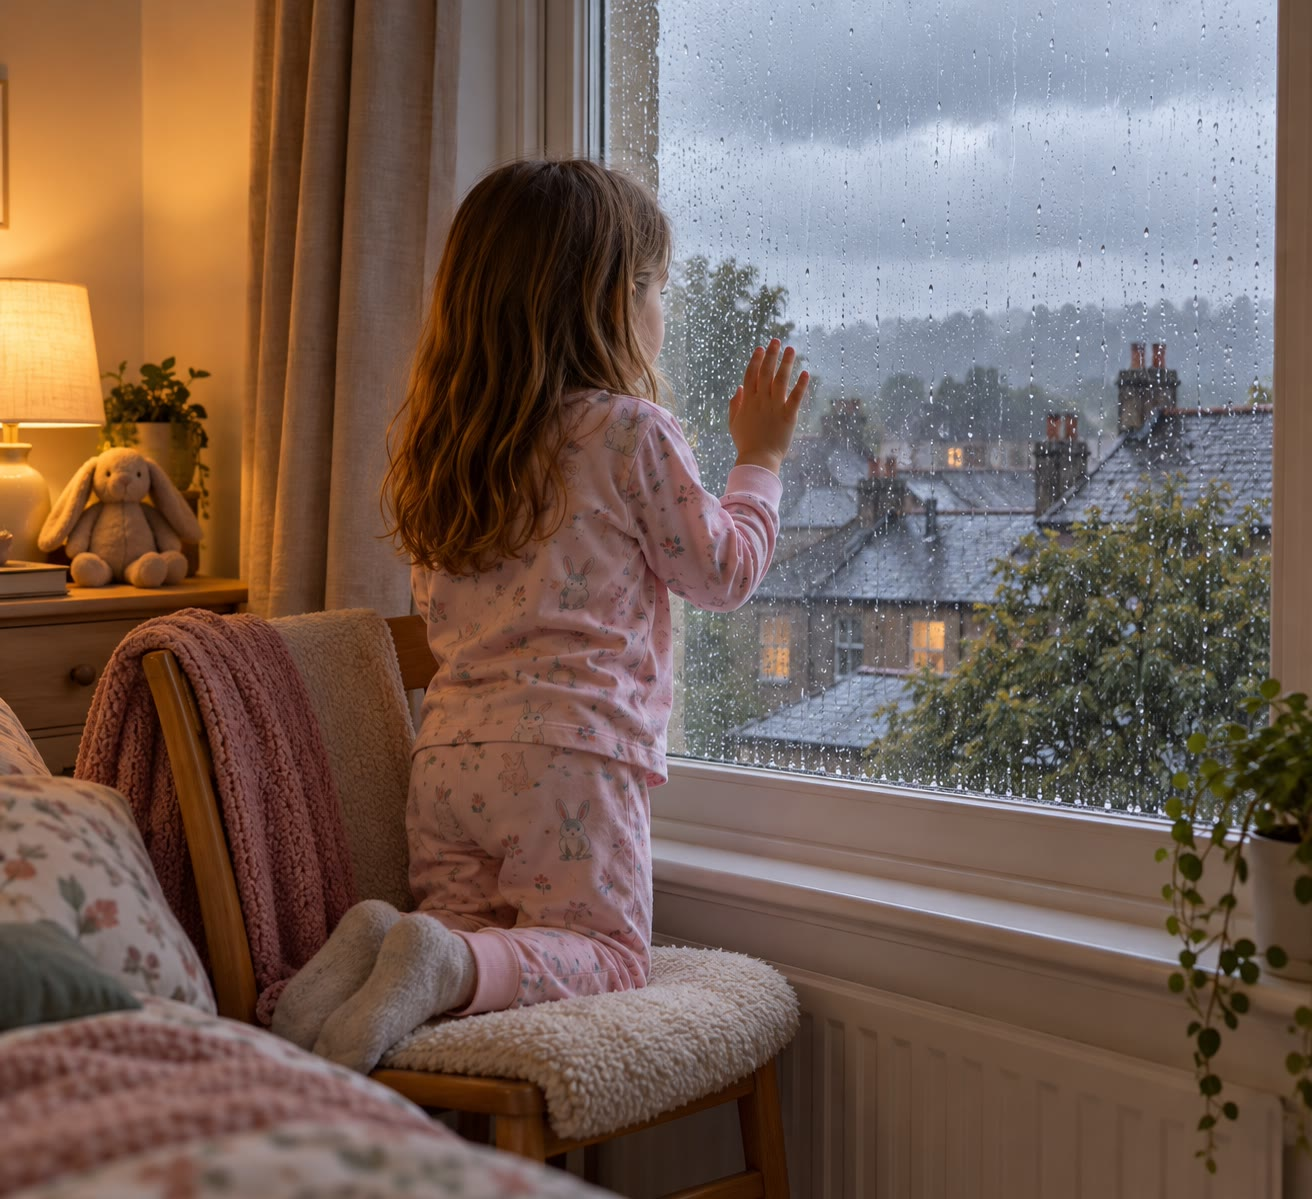
\includegraphics[width=0.72\linewidth]{images/book1/ai/g1-rainy-window.jpg}

{\small Pagi yang kelabu dan hujan, dilihat dari balik jendela.}
\end{omfigure}

\begin{recall}
Setiap pagi Matahari terbit, dan hari dimulai; setiap sore Matahari
terbenam, dan malam pun tiba. Di buku fisika kamu sudah melihat mengapa
siang berganti malam. Di bab ini kita mengamati hal lain yang selalu
berubah: \omterm{def:g1:watching-the-weather:weather}{cuaca}.
\end{recall}

\section{Apa itu cuaca?}

Ketika kita keluar rumah, kita merasakan udara di wajah kita. Udara bisa
terasa hangat atau dingin. Udara bisa diam saja, atau bisa mendorong rambut
dan baju kita: itulah angin. Kita menengadah ke langit. Langit bisa biru
dan cerah, atau tertutup awan. Kadang-kadang hujan turun dari awan,
kadang-kadang salju. Semua itu bersama-sama adalah \omterm{def:g1:watching-the-weather:weather}{cuaca}.

\begin{definition}[Cuaca]\label{def:g1:watching-the-weather:weather}
Yang disebut \emph{cuaca}\index{cuaca} adalah keadaan udara dan langit di
satu tempat pada satu saat: cerah atau berawan, kering atau hujan atau
bersalju, tenang atau berangin, hangat atau dingin.
\end{definition}

Untuk menggambarkan \omterm{def:g1:watching-the-weather:weather}{cuaca}, kita menjawab beberapa pertanyaan sederhana:
\begin{enumerate}
  \item \textbf{Seperti apa langitnya?} Apakah langit biru, dengan Matahari
        yang bersinar? Apakah ada beberapa awan, atau langit kelabu semuanya?
  \item \textbf{Adakah sesuatu yang jatuh dari langit?} Hujan? Salju? Tidak ada?
  \item \textbf{Adakah angin?} Apakah daun-daun pohon bergerak? Apakah
        bendera berkibar?
  \item \textbf{Hangat atau dingin?} Apakah kita perlu memakai mantel?
\end{enumerate}

\begin{omfigure}
\begin{minipage}[b]{0.49\linewidth}\centering
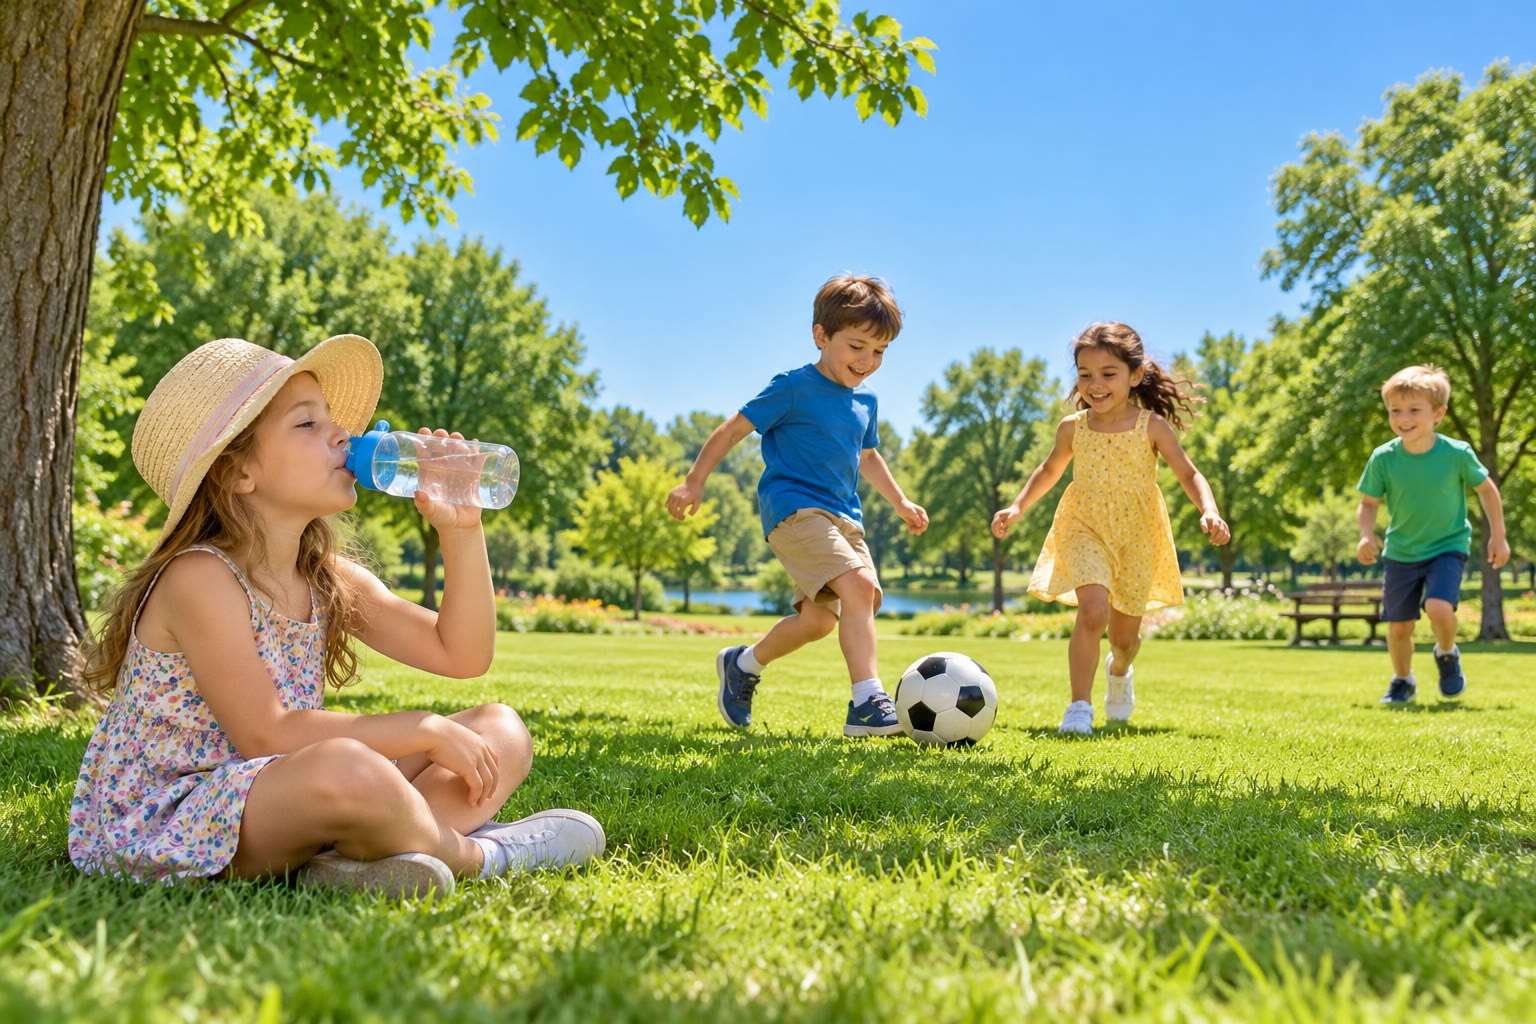
\includegraphics[width=\linewidth]{images/book1/ai/g1-sunny-park.jpg}

{\small Cerah dan hangat.}
\end{minipage}\hfill
\begin{minipage}[b]{0.49\linewidth}\centering
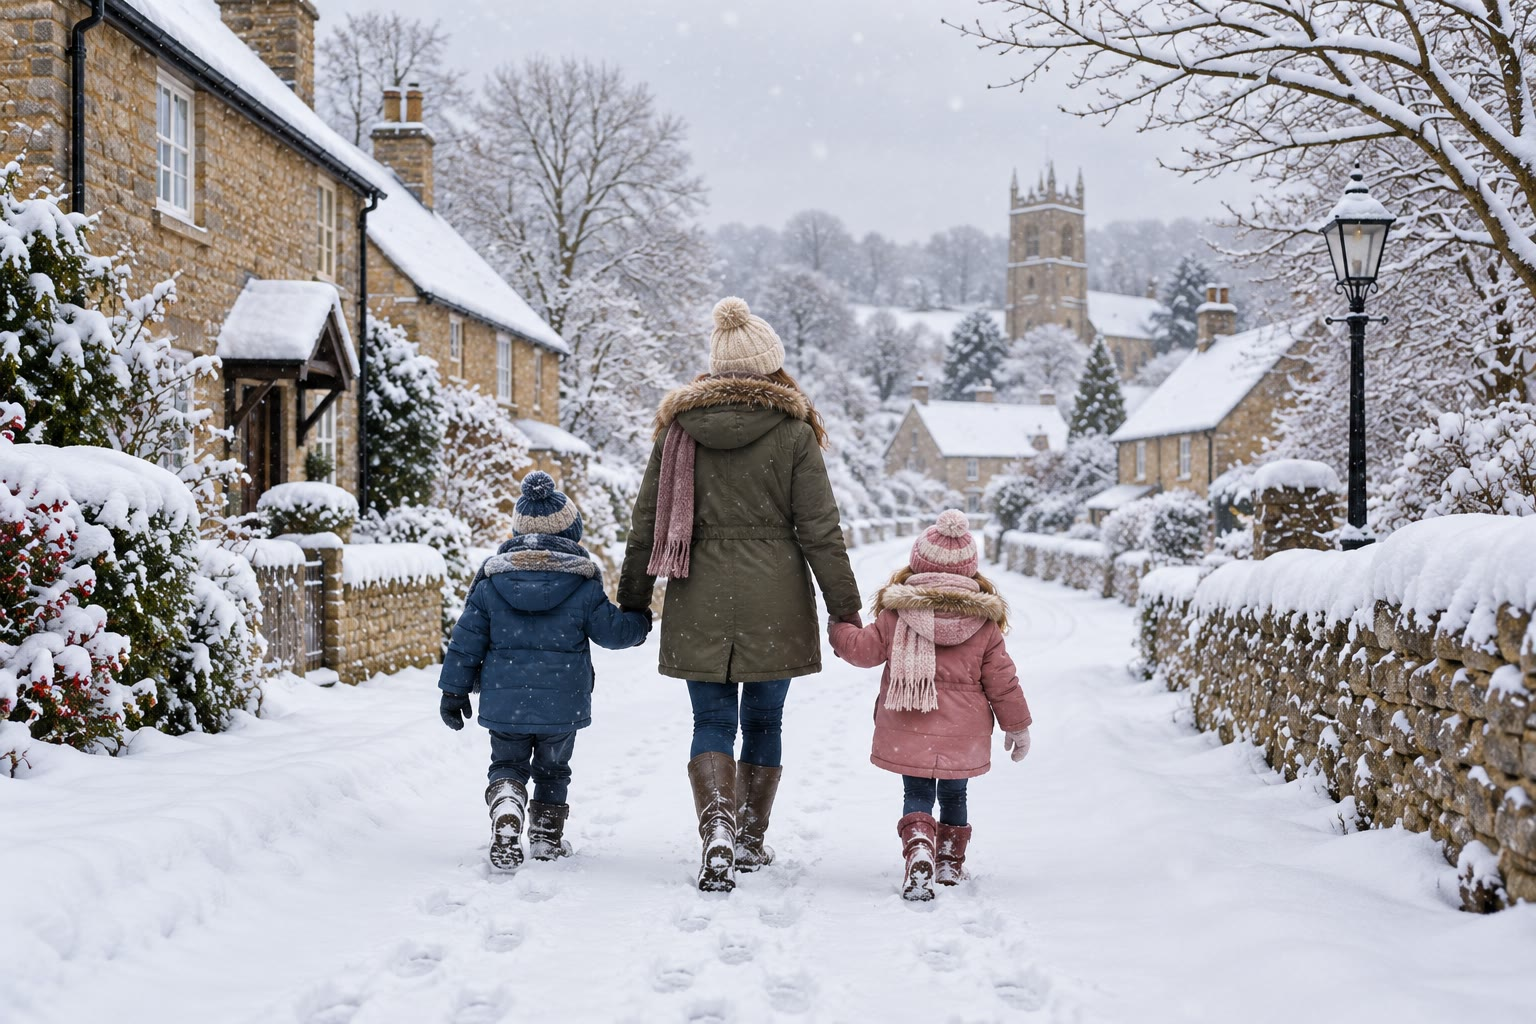
\includegraphics[width=\linewidth]{images/book1/ai/g1-snowy-street.jpg}

{\small Bersalju dan dingin.}
\end{minipage}

\medskip
\begin{minipage}[b]{0.49\linewidth}\centering
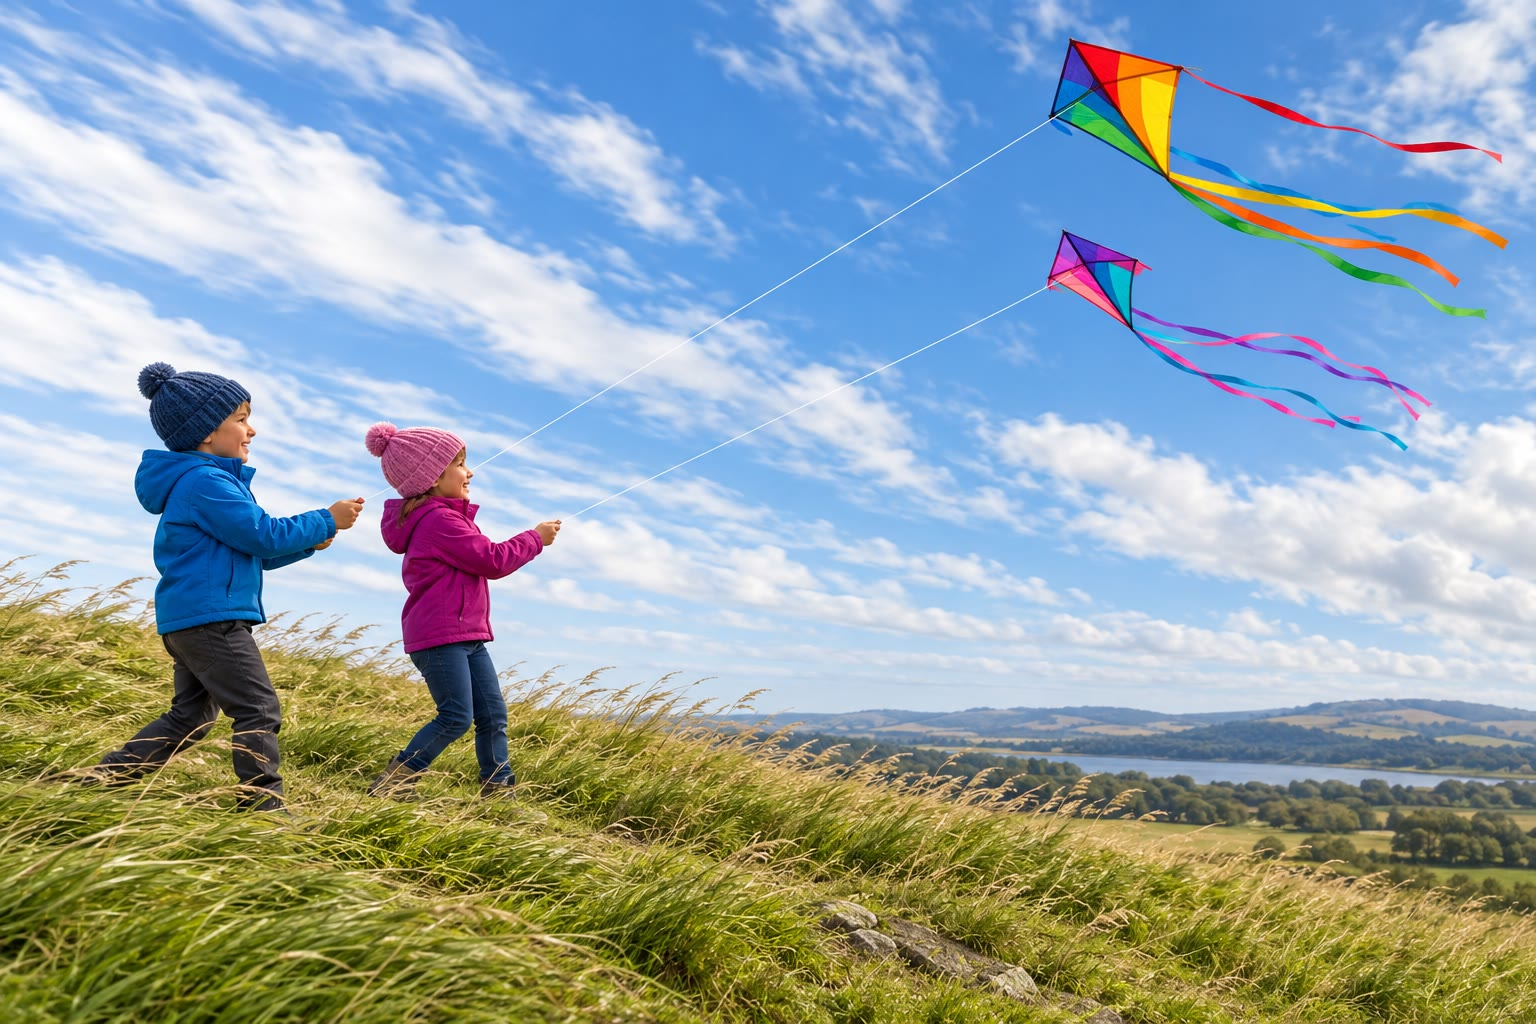
\includegraphics[width=\linewidth]{images/book1/ai/g1-windy-kites.jpg}

{\small Berangin: layang-layang terbang.}
\end{minipage}\hfill
\begin{minipage}[b]{0.49\linewidth}\centering
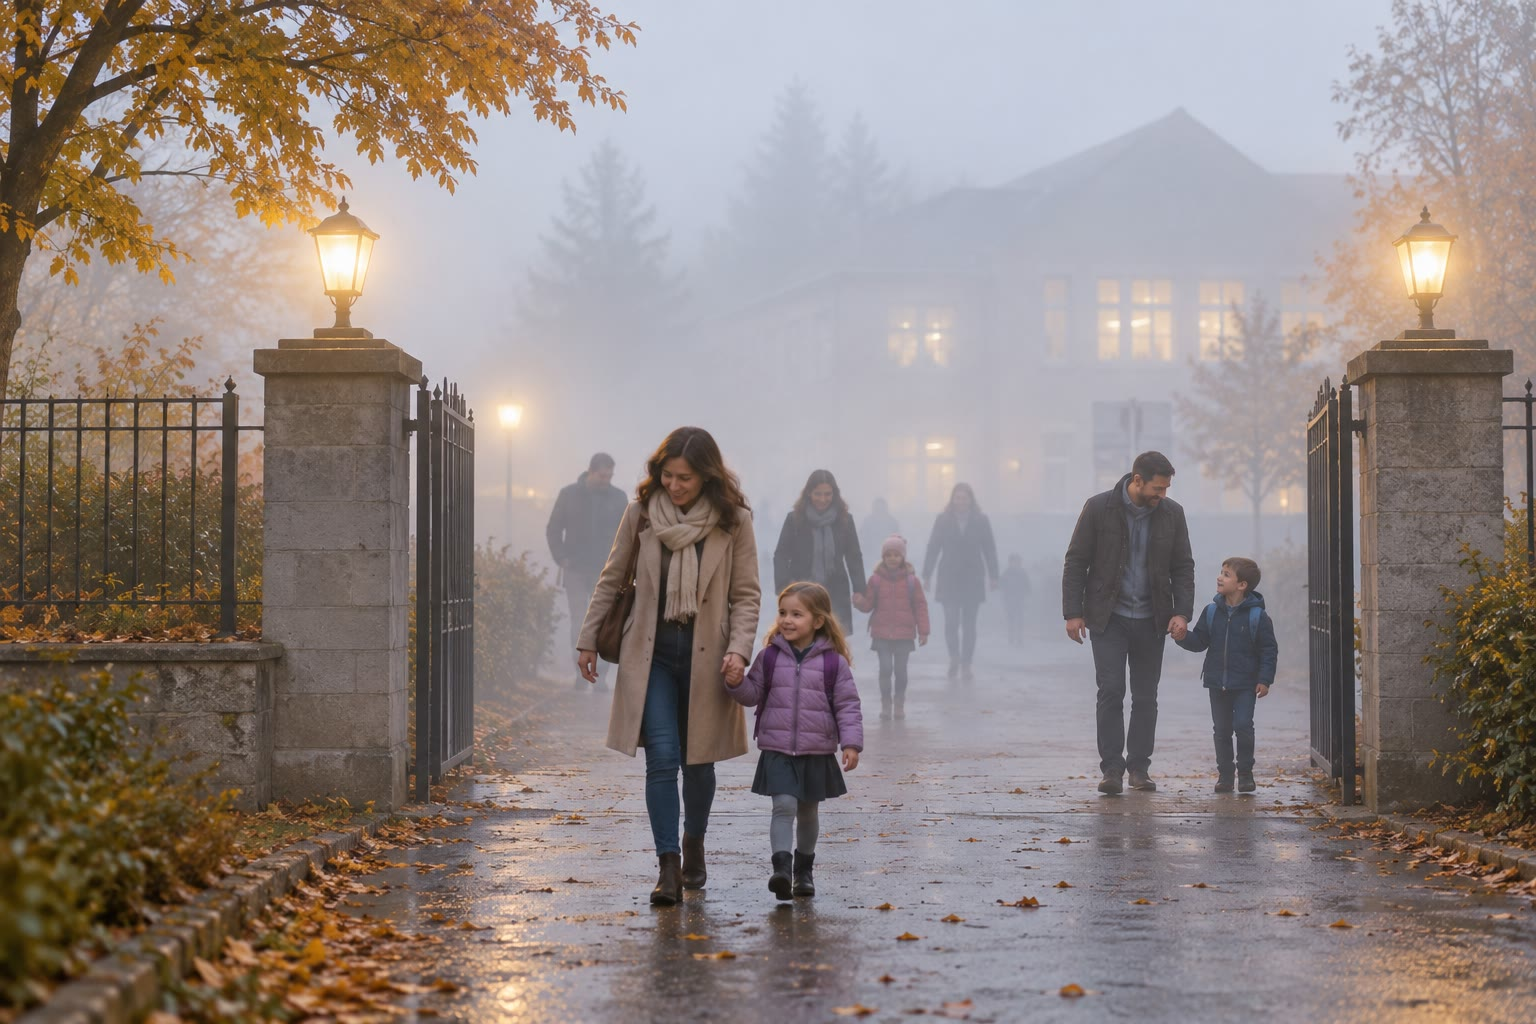
\includegraphics[width=\linewidth]{images/book1/ai/g1-foggy-school.jpg}

{\small Berkabut: kita tidak bisa melihat jauh.}
\end{minipage}
\end{omfigure}

\begin{example}[Kabut]\label{ex:g1:watching-the-weather:fog}
Pada pagi-pagi tertentu, udaranya sendiri tampak putih, dan pohon-pohon di
ujung jalan seolah menghilang. Itulah kabut. Kabut adalah awan yang
menyentuh tanah. Ketika hari mulai hangat, kabut sering kali menghilang.
\end{example}

\section{Simbol cuaca dan tabel cuaca}

Menggambarkan \omterm{def:g1:watching-the-weather:weather}{cuaca} dengan kata-kata memakan waktu lama. Orang yang
mengamati \omterm{def:g1:watching-the-weather:weather}{cuaca} memakai gambar-gambar kecil sebagai gantinya: \omterm{def:g1:watching-the-weather:weather-chart}{simbol
cuaca}. Setiap simbol mudah digambar dan mudah dikenali.

\begin{omfigure}
\begin{tikzpicture}[x=1cm, y=1cm]
  \foreach \i/\n/\t in {0/sun/cerah, 1/suncloud/cerah berawan,
      2/cloud/berawan, 3/rain/hujan, 4/shower/hujan sebentar-sebentar} {
    \pic[scale=1.25, transform shape] at (\i*2.6,0) {omwx=\n};
    \node[font=\small, align=center, text width=2.4cm] at (\i*2.6,-1.05) {\t};
  }
  \foreach \i/\n/\t in {0/snow/bersalju, 1/storm/badai petir, 2/fog/berkabut,
      3/wind/berangin} {
    \pic[scale=1.25, transform shape] at (\i*2.6+1.3,-2.6) {omwx=\n};
    \node[font=\small, align=center, text width=2.4cm] at (\i*2.6+1.3,-3.65) {\t};
  }
\end{tikzpicture}

{\small Sembilan \omterm{def:g1:watching-the-weather:weather-chart}{simbol cuaca}. Badai petir digambar dengan awan gelap dan
kilatan petir; hujan sebentar-sebentar datang dengan sinar matahari di sela-selanya.}
\end{omfigure}

\begin{definition}[Tabel cuaca]\label{def:g1:watching-the-weather:weather-chart}
Yang disebut \emph{simbol cuaca}\index{simbol cuaca} adalah gambar kecil
yang menunjukkan satu jenis \omterm{def:g1:watching-the-weather:weather}{cuaca}. Yang disebut \emph{tabel cuaca}\index{tabel cuaca}
adalah tabel tempat kita mencatat, hari demi hari, \omterm{def:g1:watching-the-weather:weather}{cuaca} yang sudah kita
lihat, dengan simbol-simbol \omterm{def:g1:watching-the-weather:weather}{cuaca}.
\end{definition}

Sebuah kelas bisa mengisi \omterm{def:g1:watching-the-weather:weather-chart}{tabel cuaca} selama satu minggu penuh. Setiap
pagi, dan sekali lagi setiap siang, seorang anak melihat ke luar dan
menggambar simbolnya di kotak yang tepat. Kita juga mencatat apakah udara
hangat atau dingin.

\begin{omfigure}
\begin{tikzpicture}[x=1cm, y=1cm]
  \def\cw{1.9}
  \foreach \d [count=\i from 0] in {Senin, Selasa, Rabu, Kamis,
      Jumat, Sabtu, Minggu}
    \node[font=\scriptsize\bfseries] at ({1.6+\i*\cw+\cw/2},0.35) {\d};
  \node[font=\scriptsize\bfseries, anchor=east] at (1.45,-0.5) {pagi};
  \node[font=\scriptsize\bfseries, anchor=east] at (1.45,-1.5) {siang};
  \node[font=\scriptsize\bfseries, anchor=east, align=right] at (1.45,-2.35) {hangat atau\\dingin?};
  \draw[black!60] (1.6,0) rectangle ({1.6+7*\cw},-2.7);
  \foreach \i in {1,...,6}
    \draw[black!60] ({1.6+\i*\cw},0.65) -- ({1.6+\i*\cw},-2.7);
  \draw[black!60] (1.6,0.65) -- ({1.6+7*\cw},0.65);
  \draw[black!60] (1.6,0.65) -- (1.6,0);
  \draw[black!60] ({1.6+7*\cw},0.65) -- ({1.6+7*\cw},0);
  \draw[black!60] (1.6,-1) -- ({1.6+7*\cw},-1);
  \draw[black!60] (1.6,-2) -- ({1.6+7*\cw},-2);
  \foreach \i/\m/\a/\w in {0/rain/rain/dingin, 1/cloud/suncloud/dingin,
      2/sun/sun/hangat, 3/sun/suncloud/hangat, 4/suncloud/shower/hangat,
      5/fog/sun/hangat, 6/cloud/rain/dingin} {
    \pic[scale=0.8, transform shape] at ({1.6+\i*\cw+\cw/2},-0.5) {omwx=\m};
    \pic[scale=0.8, transform shape] at ({1.6+\i*\cw+\cw/2},-1.5) {omwx=\a};
    \node[font=\scriptsize] at ({1.6+\i*\cw+\cw/2},-2.35) {\w};
  }
\end{tikzpicture}

{\small \omterm{def:g1:watching-the-weather:weather-chart}{Tabel cuaca} yang diisi sebuah kelas selama satu minggu di musim semi.}
\label{fig:g1:watching-the-weather:chart}
\end{omfigure}

\begin{method}[Membaca tabel cuaca]\label{met:g1:watching-the-weather:read}
Untuk membaca \omterm{def:g1:watching-the-weather:weather-chart}{tabel cuaca}:
\begin{enumerate}
  \item carilah kolom hari yang kamu inginkan;
  \item lihatlah barisnya: pagi, atau siang;
  \item sebutkan \omterm{def:g1:watching-the-weather:weather}{cuaca} yang ditunjukkan simbolnya.
\end{enumerate}
Untuk mengetahui berapa hari yang cerah, telusurilah satu baris dengan
jarimu dan hitunglah simbol mataharinya.
\end{method}

\begin{example}[Membaca tabel kelas]\label{ex:g1:watching-the-weather:read}
Pada tabel kelas ini, Senin pagi hujan dan dingin. Hari Rabu cerah
sepanjang hari. Hari Sabtu kabut di pagi hari berganti dengan sinar
matahari di siang hari. Pada pagi-pagi dalam minggu itu, kelas tersebut
menggambar matahari pada 2 hari: Rabu dan Kamis.
\end{example}

\section{Cuaca berubah-ubah}

\omterm{def:g1:watching-the-weather:weather}{Cuaca} tidak tetap sama. \omterm{def:g1:watching-the-weather:weather}{Cuaca} berubah dalam satu hari, dari satu hari ke
hari berikutnya, dan sepanjang tahun.

\begin{itemize}
  \item \textbf{Dalam satu hari.} Pagi yang kelabu bisa berubah menjadi
        siang yang cerah. Pagi yang biru bersih bisa berakhir dengan badai.
        Pada pagi-pagi buta dan pada malam hari, udara biasanya lebih sejuk
        daripada siang hari.
  \item \textbf{Dari satu hari ke hari berikutnya.} Lihatlah tabel kelas:
        tidak ada dua hari dalam minggu itu yang persis sama.
  \item \textbf{Sepanjang tahun.} Di musim panas hari-hari biasanya hangat,
        dan di musim dingin biasanya dingin; di banyak tempat salju turun
        hanya di musim dingin. Buku fisika menjelaskan mengapa musim-musim
        datang kembali setiap tahun.
\end{itemize}

\begin{omfigure}
\begin{tikzpicture}[x=1cm, y=1cm]
  \draw[black!50, line width=0.8pt, -{Stealth[length=2.5mm]}] (0,0) -- (12.2,0);
  \foreach \x/\n/\t/\h in {0.9/fog/pagi buta/sejuk, 3.5/suncloud/pagi/sedang,
      6.1/sun/siang/hangat, 8.7/storm/sore/hangat dan berbadai,
      11.2/suncloud/malam/lebih sejuk} {
    \pic[scale=1.1, transform shape] at (\x,0.85) {omwx=\n};
    \fill[black!60] (\x,0) circle (1.5pt);
    \node[font=\scriptsize\bfseries, below] at (\x,-0.12) {\t};
    \node[font=\scriptsize, below] at (\x,-0.5) {\h};
  }
\end{tikzpicture}

{\small Satu hari di musim panas, dari pagi sampai malam: \omterm{def:g1:watching-the-weather:weather}{cuacanya} berubah
lima kali.}
\label{fig:g1:watching-the-weather:day}
\end{omfigure}

\begin{omfigure}
\begin{tikzpicture}[x=1cm, y=1cm]
  \foreach \i/\s/\c/\g/\w/\gr in {0/musim semi/green!55!black/pink!60/suncloud/green!35,
      1/musim panas/green!45!black/green!50!black/sun/green!35,
      2/musim gugur/orange!80!black/orange!70/rain/green!25!brown!30,
      3/musim dingin/black!55/white/snow/white} {
    \begin{scope}[shift={(\i*3.15,0)}]
      \draw[black!30, rounded corners=3pt, fill=ocBlue!6] (-1.4,-0.45) rectangle (1.4,3.05);
      \fill[\gr] (-1.4,-0.45) rectangle (1.4,0);
      \draw[black!25] (-1.4,0) -- (1.4,0);
      \fill[brown!60!black] (-0.09,0) rectangle (0.09,1.0);
      \draw[brown!60!black, line width=1.6pt] (0,0.75) -- (-0.5,1.35);
      \draw[brown!60!black, line width=1.6pt] (0,0.9) -- (0.45,1.45);
      \ifnum\i<3
        \fill[\c, opacity=0.85] (0,1.55) circle (0.72);
        \ifnum\i=0 \foreach \a in {20,80,140,200,260,320} \fill[\g] (0,1.55) ++(\a:0.45) circle (0.09); \fi
        \ifnum\i=2 \foreach \x/\y in {-0.9/0.15,0.7/0.3,0.95/0.1} \fill[\g] (\x,\y) circle (0.07); \fi
      \else
        \draw[white, line width=2.4pt] (-0.5,1.35) -- (-0.35,1.17);
        \draw[white, line width=2.4pt] (0.45,1.45) -- (0.3,1.27);
      \fi
      \pic[scale=0.8, transform shape] at (0.95,2.55) {omwx=\w};
      \node[font=\small\bfseries] at (0,-0.75) {\s};
    \end{scope}
  }
\end{tikzpicture}

{\small Pohon yang sama dalam empat musim: berbunga di musim semi, berdaun
hijau lebat di musim panas, daunnya yang jingga berguguran di musim gugur,
dahannya gundul dan bersalju di musim dingin.}
\label{fig:g1:watching-the-weather:seasons}
\end{omfigure}

\begin{remark}[Dari mana angin datang]\label{rem:g1:watching-the-weather:wind}
Kita tidak bisa melihat angin, tetapi kita bisa melihat apa yang
dilakukannya. Bendera, kantong angin, atau asap dari cerobong didorong
oleh angin: semuanya menunjuk ke arah angin pergi, jadi angin datang dari
sisi yang berlawanan.
\end{remark}

\begin{omfigure}
\begin{tikzpicture}[x=1cm, y=1cm]
  % ground
  \fill[green!30!omLithAlluv] (-0.4,-0.1) rectangle (8.4,0);
  % windsock on a pole
  \draw[black!70, line width=1.2pt] (1,0) -- (1,3.2);
  \fill[orange!85, draw=black!60] (1,3.15) -- (3.4,2.95) -- (3.4,2.55) -- (1,2.45) -- cycle;
  \fill[white] (1.6,3.1) -- (2.2,3.05) -- (2.2,2.5) -- (1.6,2.47) -- cycle;
  \fill[white] (2.8,3.0) -- (3.4,2.95) -- (3.4,2.55) -- (2.8,2.53) -- cycle;
  \draw[black!60] (1,3.15) -- (3.4,2.95) -- (3.4,2.55) -- (1,2.45);
  % flag
  \draw[black!70, line width=1.2pt] (5.4,0) -- (5.4,3.2);
  \fill[ocBlue!70, draw=black!60] (5.4,3.15) .. controls (6.0,3.3) and (6.4,2.9) .. (7.1,3.05)
     -- (7.1,2.35) .. controls (6.4,2.2) and (6.0,2.6) .. (5.4,2.45) -- cycle;
  % wind arrows
  \foreach \y in {1.0,1.6}
    \draw[omWxRain, line width=1.4pt, -{Stealth[length=3mm]}] (-0.3,\y) -- (0.7,\y);
  \node[font=\small, align=right, anchor=east] at (-0.45,1.3) {angin\\datang dari sini};
  \draw[black!60, -{Stealth[length=2mm]}] (4.1,2.75) -- (4.9,2.75);
  \node[font=\small, align=left, anchor=west] at (7.5,2.7) {bendera dan kantong\\angin menunjuk ke\\arah angin pergi};
\end{tikzpicture}

{\small Kantong angin dan bendera pada hari yang berangin. Angin bertiup
dari kiri ke kanan.}
\end{omfigure}

\section{Mengapa kita mengamati cuaca?}

Banyak orang perlu tahu bagaimana \omterm{def:g1:watching-the-weather:weather}{cuaca} nanti.
\begin{itemize}
  \item \textbf{Petani} mengamati langit sebelum memotong rumput kering:
        hujan bisa merusaknya. Di musim semi mereka khawatir akan malam
        yang membeku, yang bisa mematikan tanaman muda.
  \item \textbf{Pelaut dan nelayan} mengamati angin: angin yang kencang
        membuat ombak besar, dan perahu-perahu tetap tinggal di pelabuhan.
  \item \textbf{Pilot} perlu tahu tentang kabut, badai, dan angin sebelum
        pesawat terbang lepas landas.
  \item \textbf{Sebuah kelas} yang akan bertamasya ke hutan ingin tahu
        apakah harus membawa jas hujan atau topi pantai.
\end{itemize}
Setiap hari, orang-orang yang disebut ahli meteorologi mengamati \omterm{def:g1:watching-the-weather:weather}{cuaca} di
seluruh dunia dan memberi tahu kita, lewat radio, televisi, atau ponsel,
bagaimana kira-kira \omterm{def:g1:watching-the-weather:weather}{cuaca} pada hari-hari berikutnya.

\begin{example}[Tanda-tanda di langit]\label{ex:g1:watching-the-weather:signs}
Jauh sebelum ada radio dan ponsel, orang sudah belajar membaca langit.
Ketika awan-awan putih yang kecil tumbuh pada siang hari menjadi menara
yang tinggi dan gelap, hujan lebat atau badai petir akan datang. Ketika
angin berbalik arah dan langit perlahan-lahan tertutup selubung kelabu,
hujan sering turun beberapa jam kemudian. Tanda-tanda ini tidak selalu
benar, tetapi sering kali berguna.
\end{example}

\section{Berpakaian sesuai cuaca}

Sekarang Lena bisa menjawab pertanyaannya. Hari ini hujan dan dingin, jadi
ia akan memakai jas hujan dan sepatu botnya. Besok \omterm{def:g1:watching-the-weather:weather}{cuacanya} mungkin lain,
dan ia akan memilih lagi.

\begin{omfigure}
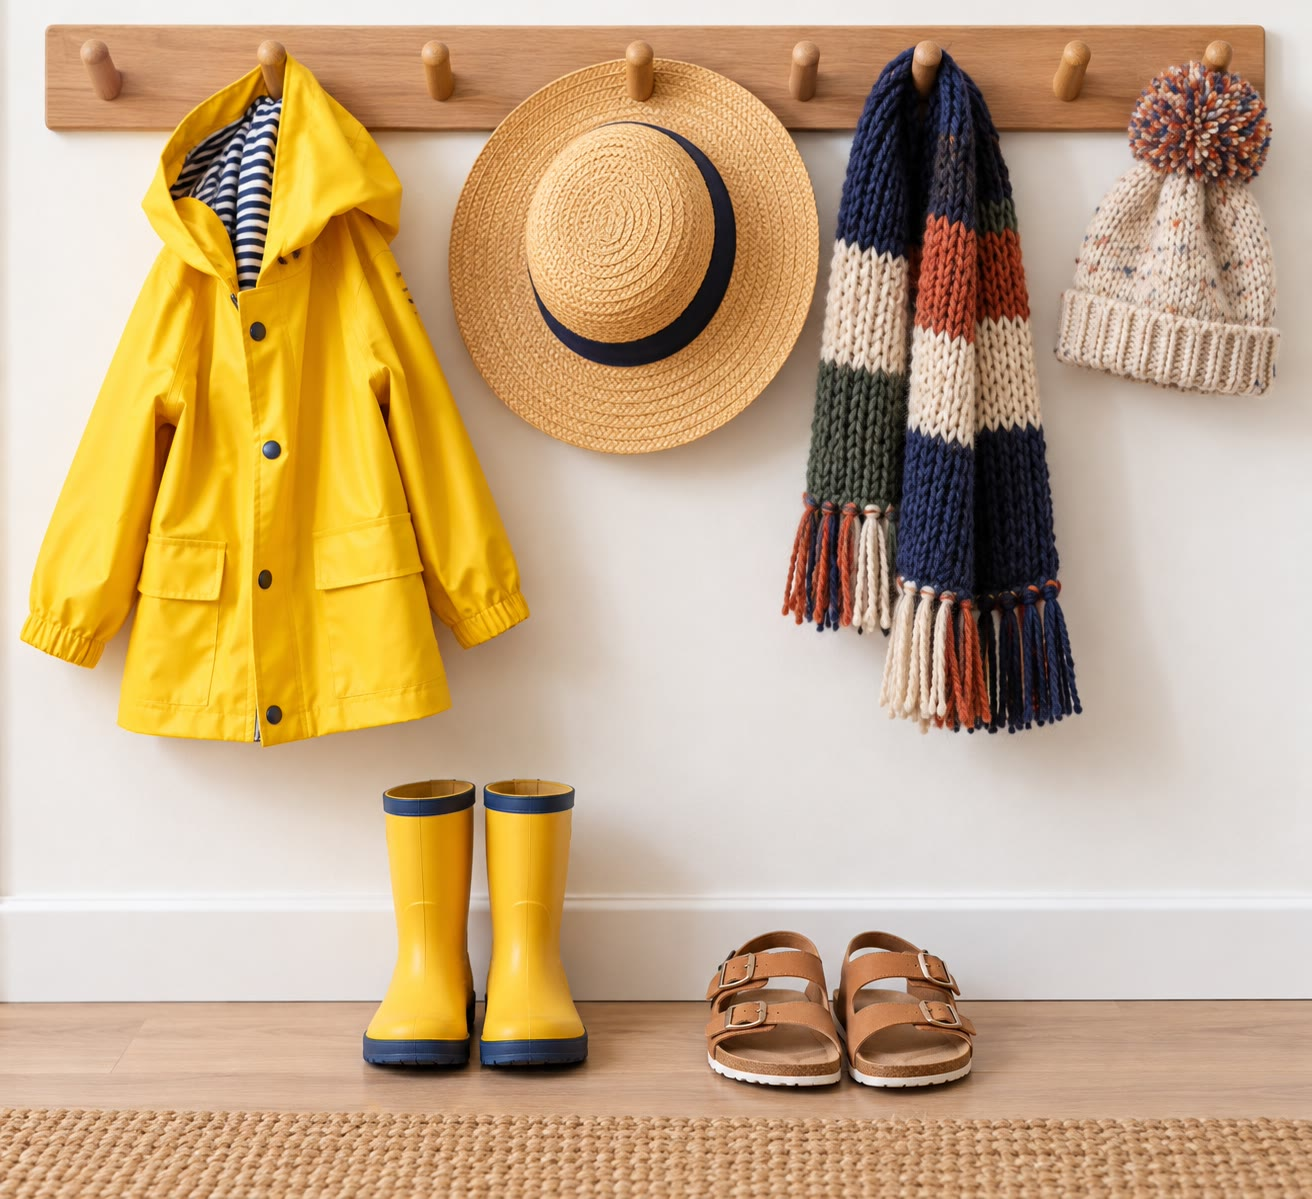
\includegraphics[width=0.66\linewidth]{images/book1/ai/g1-coat-pegs.jpg}

{\small Pakaian untuk setiap jenis \omterm{def:g1:watching-the-weather:weather}{cuaca}: jas hujan, topi pantai, syal dan
topi hangat, sepatu bot dan sandal.}
\end{omfigure}

\begin{method}[Memilih pakaian sesuai cuaca]\label{met:g1:watching-the-weather:clothes}
Lihatlah langit dan rasakan udaranya, lalu:
\begin{itemize}
  \item hujan atau hujan sebentar-sebentar: jas hujan atau payung, dan
        sepatu bot;
  \item dingin atau salju: mantel hangat, syal, topi, dan sarung tangan;
  \item sinar matahari terik dan panas: topi pantai, baju yang tipis, dan
        air untuk diminum;
  \item angin: mantel yang tertutup rapat; payung tidak banyak membantu.
\end{itemize}
\end{method}

\begin{safety}
\textbf{Jangan pernah menatap langsung ke Matahari}, sesaat pun jangan, dan
jangan pernah melalui kacamata, teropong, atau kamera: matamu bisa rusak
selamanya. Ketika ada badai petir, tetaplah di dalam rumah atau di dalam
mobil, jauhilah pohon-pohon tinggi dan air, dan tunggulah sampai badainya
berlalu.
\end{safety}

\section{Latihan}

\begin{exercise}[$\star$]\label{exo:g1:watching-the-weather:1}
Gambarlah simbol untuk setiap jenis \omterm{def:g1:watching-the-weather:weather}{cuaca}: cerah; hujan; bersalju; berawan.
\end{exercise}

\begin{exercise}[$\star$]\label{exo:g1:watching-the-weather:2}
Bagaimana \omterm{def:g1:watching-the-weather:weather}{cuaca} pada setiap gambar dari keempat gambar di subbab ``Apa itu
\omterm{def:g1:watching-the-weather:weather}{cuaca}?''? Pakailah satu atau dua kata untuk masing-masing.
\end{exercise}

\begin{exercise}[$\star$]\label{exo:g1:watching-the-weather:3}
Lihatlah \omterm{def:g1:watching-the-weather:weather-chart}{tabel cuaca} kelas. Bagaimana \omterm{def:g1:watching-the-weather:weather}{cuacanya} pada Selasa pagi? Pada
Jumat siang? Pada Minggu siang?
\end{exercise}

\begin{exercise}[$\star$]\label{exo:g1:watching-the-weather:4}
Pada \omterm{def:g1:watching-the-weather:weather-chart}{tabel cuaca} kelas, pada hari apa \omterm{def:g1:watching-the-weather:weather}{cuacanya} cerah di pagi hari dan juga
di siang hari?
\end{exercise}

\begin{exercise}[$\star$]\label{exo:g1:watching-the-weather:5}
Pasangkan setiap pakaian dengan satu \omterm{def:g1:watching-the-weather:weather}{cuaca}: topi pantai; sepatu bot dan
jas hujan; syal dan sarung tangan. \omterm{def:g1:watching-the-weather:weather}{Cuacanya} adalah: dingin dan bersalju;
panas dan cerah; hujan.
\end{exercise}

\begin{exercise}[$\star$]\label{exo:g1:watching-the-weather:6}
Lena berkata: ``Lihat, benderanya berkibar-kibar!'' Bagaimana \omterm{def:g1:watching-the-weather:weather}{cuacanya}?
\end{exercise}

\begin{exercise}[$\star$]\label{exo:g1:watching-the-weather:7}
Benar atau salah? Jelaskan.
\begin{enumerate}
  \item \omterm{def:g1:watching-the-weather:weather}{Cuaca} selalu sama pada pagi dan siang hari.
  \item Kabut adalah awan yang menyentuh tanah.
  \item Aturan ``jangan pernah melihat Matahari, sebelah mata pun jangan'' adalah aturan yang baik.
\end{enumerate}
\end{exercise}

\begin{exercise}[$\star\star$]\label{exo:g1:watching-the-weather:8}
Pada \omterm{def:g1:watching-the-weather:weather-chart}{tabel cuaca} kelas, hitunglah siang-siang yang hujan atau hujan
sebentar-sebentar. Hitunglah hari-hari yang dingin. Apakah minggu itu
lebih sering hangat atau lebih sering dingin?
\end{exercise}

\begin{exercise}[$\star\star$]\label{exo:g1:watching-the-weather:9}
Inilah yang dilihat Sam dari jendelanya selama satu hari: di pagi hari,
langit kelabu; pada waktu makan siang, tetes-tetes air di jendela; di malam
hari, langit biru dengan beberapa awan. Gambarlah ketiga \omterm{def:g1:watching-the-weather:weather-chart}{simbol cuacanya}
dengan urutan yang benar.
\end{exercise}

\begin{exercise}[$\star\star$]\label{exo:g1:watching-the-weather:10}
Pada gambar kantong angin dan bendera, angin datang dari kiri. Pada hari
lain, sebuah bendera menunjuk ke kiri. Dari sisi mana angin datang pada
hari itu?
\end{exercise}

\begin{exercise}[$\star\star$]\label{exo:g1:watching-the-weather:11}
Lihatlah gambar pohon yang sama dalam empat musim. Pada musim apa pohon
itu tidak berdaun? Pada musim apa pohon itu berbunga? \omterm{def:g1:watching-the-weather:weather-chart}{Simbol cuaca} apa
yang digambar untuk musim dingin, dan mengapa simbol itu cocok dengan
musim tersebut?
\end{exercise}
